%%% Hlavní soubor. Zde se definují základní parametry a odkazuje se na ostatní části. %%%

%% Verze pro jednostranný tisk:
% Okraje: levý 40mm, pravý 25mm, horní a dolní 25mm
% (ale pozor, LaTeX si sám přidává 1in)
\documentclass[12pt,a4paper]{report}
\setlength\textwidth{145mm}
\setlength\textheight{247mm}
\setlength\oddsidemargin{15mm}
\setlength\evensidemargin{15mm}
\setlength\topmargin{0mm}
\setlength\headsep{0mm}
\setlength\headheight{0mm}
% \openright zařídí, aby následující text začínal na pravé straně knihy
\let\openright=\clearpage

%% Pokud tiskneme oboustranně:
% \documentclass[12pt,a4paper,twoside,openright]{report}
% \setlength\textwidth{145mm}
% \setlength\textheight{247mm}
% \setlength\oddsidemargin{15mm}
% \setlength\evensidemargin{0mm}
% \setlength\topmargin{0mm}
% \setlength\headsep{0mm}
% \setlength\headheight{0mm}
% \let\openright=\cleardoublepage

%% Použité kódování znaků: obvykle latin2, cp1250 nebo utf8:
\usepackage[utf8]{inputenc}

%% Ostatní balíčky
\usepackage{multirow}
\usepackage{amsthm}

\usepackage{graphicx}
\usepackage{wrapfig}
\graphicspath{ {img/} }

\usepackage{algorithm,algorithmicx,algpseudocode}
\usepackage{minted}

\usepackage[toc,title,header]{appendix}

%% Balicky pro pekne vytisteni zdrojoveho kodu
\usepackage{listings}
\usepackage{xcolor}
\colorlet{punct}{red!60!black}
\definecolor{background}{HTML}{FFFFFF}
\definecolor{delim}{RGB}{20,105,176}
\colorlet{numb}{magenta!60!black}
\lstdefinelanguage{json}{
    basicstyle=\normalfont\ttfamily,
    numbers=none,
    numberstyle=\scriptsize,
    stepnumber=1,
    numbersep=8pt,
    showstringspaces=false,
    breaklines=true,
    frame=none,
    backgroundcolor=\color{background},
}

% Nastavení číslování i pro subsubsection
\setcounter{secnumdepth}{4}

%% Balíček hyperref, kterým jdou vyrábět klikací odkazy v PDF,
%% ale hlavně ho používáme k uložení metadat do PDF (včetně obsahu).
%% POZOR, nezapomeňte vyplnit jméno práce a autora.
\usepackage[unicode]{hyperref}   % Musí být za všemi ostatními balíčky
\hypersetup{pdftitle=Optimization of Processing of Data Files in System DIRAC}
\hypersetup{pdfauthor=Martin Adam}

%%% Drobné úpravy stylu

% Tato makra přesvědčují mírně ošklivým trikem LaTeX, aby hlavičky kapitol
% sázel příčetněji a nevynechával nad nimi spoustu místa. Směle ignorujte.
\makeatletter
\def\@makechapterhead#1{
  {\parindent \z@ \raggedright \normalfont
   \Huge\bfseries \thechapter. #1
   \par\nobreak
   \vskip 20\p@
}}
\def\@makeschapterhead#1{
  {\parindent \z@ \raggedright \normalfont
   \Huge\bfseries #1
   \par\nobreak
   \vskip 20\p@
}}
\makeatother

% Toto makro definuje kapitolu, která není očíslovaná, ale je uvedena v obsahu.
\def\chapwithtoc#1{
\chapter*{#1}
\addcontentsline{toc}{chapter}{#1}
}

\begin{document}

% Trochu volnější nastavení dělení slov, než je default.
\lefthyphenmin=2
\righthyphenmin=2

%%% Titulní strana práce

\pagestyle{empty}
\begin{center}

\large

Charles University in Prague

\medskip

Faculty of Mathematics and Physics

\vfill

{\bf\Large BACHELOR THESIS}

\vfill

\centerline{\mbox{\includegraphics[width=60mm]{logo.eps}}}

\vfill
\vspace{5mm}

{\LARGE Martin Adam}

\vspace{15mm}

% Název práce přesně podle zadání
{\LARGE\bfseries Optimization of Processing of Data Files in System DIRAC}

\vfill

% Název katedry nebo ústavu, kde byla práce oficiálně zadána
% (dle Organizační struktury MFF UK)
Department of Software Engineering

\vfill

\begin{tabular}{rl}

Supervisor of the bachelor thesis: & doc. RNDr. Irena Holubová, Ph.D. \\
\noalign{\vspace{2mm}}
Study programme: & Computer Science \\
\noalign{\vspace{2mm}}
Specialization: &  Administration of Computer Systems \\
\end{tabular}

\vfill

% Zde doplňte rok
Prague 2015

\end{center}

\newpage

%%% Následuje vevázaný list -- kopie podepsaného "Zadání bakalářské práce".
%%% Toto zadání NENÍ součástí elektronické verze práce, nescanovat.

%%% Na tomto místě mohou být napsána případná poděkování (vedoucímu práce,
%%% konzultantovi, tomu, kdo zapůjčil software, literaturu apod.)

\openright

\noindent
I would like to thank my supervisor, doc. RNDr. Irena Holubová, Ph.D., for patience and advice when
writing this thesis. 

I would also want to thank Dr. Andrei Tsaregorodtsev, the DIRAC product manager for finding me a suitable
task I could work on during my thesis and to continuous encouragement and help during my work. 
Further, I thank RNDr. Jiří Chudoba, Ph.D. for providing me with a suitable testing
environment in the computing center of the Institute of Physics of the Czech Academy of Sciences.

Finally my thanks belong to my parents for helping me enhance the text of this thesis and last but not least my 
girlfriend Annie for her great patience and support.

\newpage

%%% Strana s čestným prohlášením k bakalářské práci

\vglue 0pt plus 1fill

\noindent
I declare that I carried out this bachelor thesis independently, and only with the cited
sources, literature and other professional sources.

\medskip\noindent
I understand that my work relates to the rights and obligations under the Act No.
121/2000 Coll., the Copyright Act, as amended, in particular the fact that the Charles
University in Prague has the right to conclude a license agreement on the use of this
work as a school work pursuant to Section 60 paragraph 1 of the Copyright Act.

\vspace{10mm}

\hbox{\hbox to 0.5\hsize{%
In ........ date ............
\hss}\hbox to 0.5\hsize{%
signature of the author
\hss}}

\vspace{20mm}
\newpage

%%% Povinná informační strana bakalářské práce

\vbox to 0.5\vsize{
\setlength\parindent{0mm}
\setlength\parskip{5mm}

Název práce:
Optimalizace Zpracování Dat v Systému DIRAC
% přesně dle zadání

Autor:
Martin Adam

Katedra:  % Případně Ústav:
Katedra softwarového inženýrství
% dle Organizační struktury MFF UK

Vedoucí bakalářské práce:
doc. RNDr. Irena Holubová, Ph.D.
% dle Organizační struktury MFF UK, případně plný název pracoviště mimo MFF UK

Abstrakt:
V této práci je rozšířen DIRAC File Catalog (DFC) o modul DatasetManager přidávající funkcionalitu datasetů 
definovaných dotazem nad metadaty. K vylepšení práce s dotazy v kódu systému, je vyvinuta nová třída MetaQuery,
která shlukuje obslužné metody a přidává normalizaci a optimalizaci dotazu na vstupu. Jazyk vyjadřující 
dotazy byl také rozšířen přidáním možnosti používat logické spojky a závorky. 

Druhá část práce se zabývá testováním hypotézy, že použití NoSQL databáze jako back-end pro metadatovou část
DFC by přineslo vylepšení výkonu vyhledávání. Několik NoSQL databází je otestováno na datech podobných 
produkčním datům používaných systémem DIRAC. Nejvýkonější databáze na základě testů je pak připojena k DFC 
použitím nového specializovaného rozhraní.

Klíčová slova:
System DIRAC, NoSQL databases, efficient processing of data files, metadata querying

\vss}\nobreak\vbox to 0.49\vsize{
\setlength\parindent{0mm}
\setlength\parskip{5mm}

Title:
Optimization of Processing of Data Files in System DIRAC
% přesný překlad názvu práce v angličtině

Author:
Martin Adam

Department:
Department of Software Engineering
% dle Organizační struktury MFF UK v angličtině

Supervisor:
doc. RNDr. Irena Holubová, Ph.D.
% dle Organizační struktury MFF UK, případně plný název pracoviště
% mimo MFF UK v angličtině

Abstract:
In this thesis the DIRAC File Catalog (DFC) is extended by adding a DatasetManager module thus adding support
for datasets based on metadata queries. To improve the metaquery handling in the code a new class MetaQuery 
was implemented, which bundles the handling methods as well as adds normalization and optimization of the user 
input. Also the metaquery language was extended enabling logical operators and parenthesis. 

In the second part of the thesis the hypothesis that connecting the metadata part of the DIRAC File Catalog to a 
NoSQL database could improve metaquery performance is evaluated. Several databases are tested and the best 
performing is then connected using an interface module to the DFC.

Keywords:
System DIRAC, NoSQL databases, efficient processing of data files, metadata querying

\vss}

\newpage

%%% Strana s automaticky generovaným obsahem bakalářské práce. U matematických
%%% prací je přípustné, aby seznam tabulek a zkratek, existují-li, byl umístěn
%%% na začátku práce, místo na jejím konci.

\openright
\pagestyle{plain}
\setcounter{page}{1}
\tableofcontents

%%% Jednotlivé kapitoly práce jsou pro přehlednost uloženy v samostatných souborech
\chapter*{Introduction}
\addcontentsline{toc}{chapter}{Introduction}

\section*{The Worldwide LHC Computing Grid}

In the past decade the scientific research collaborations, as well as the
commercial world, have witnessed the start of a  period  of  explosive
data growth. The expressions like "Data Tsunami" or "Big Data" became widespread
and entered a standard terminology. The scientific collaborations developed a
world leading expertise in building and operating very large scale infrastructures for
handling unprecedented and ever growing volumes of data to be processed and analyzed~\cite{OSC}.  
One of the most important scientific communities,
for which these abilities became essential, is the High Energy Physics (HEP) community of 
the experiments at the Large Hadron
Collider (LHC) at CERN\footnote{European Organization for Nuclear Research 
(name derived from Conseil Européen pour la Recherche Nucléaire) -- European research organization that operates 
the largest particle physics laboratory in the world.}.

Physicists collide particles accelerated to enormous energies to get at very short scales, which enables them to
reveal at the microscopic level the basic ingredients of the matter and their interactions. 
On the edge of our millennium their ultimate instrument is the LHC, colliding protons or 
atomic nuclei. In each 
collision debris of tens of thousands of new particles are created which have to be registered in huge detectors 
and carefully analyzed for signs of new physical phenomena. The collisions take part at four interaction areas, 
where the detectors (ATLAS, ALICE, CMS and LHCb) were built. Each experiment collects huge volumes of data that have
to be stored, remaining accessible to many groups of physicist scattered all around the globe.

The volumes of collected data are larger than
%On the edge of our millennium scientists working on the LHC were expecting enormous volumes 
%of data, larger than 
any single computing center within the LHC collaboration could handle, so the concept of 
distributed data management was conceived. In 2001 the CERN Council approved the start of an international 
collaborative project that consists of a grid-based computer network infrastructure, the Worldwide LHC Computing 
Grid (WLCG)~\cite{happyBday}. 

\begin{wrapfigure}{L}{0.6\textwidth}
\centering
\includegraphics[width=0.55\textwidth]{Tiers.pdf}
\caption{The WLCG Tier-1 centers with CERN Tier-0 in the middle}
\label{fig:WLCG}
\end{wrapfigure}

The WLCG has a hierarchical architecture, where participating sites are categorized -- according to the resources 
and services they provide -- into four importance levels called Tiers. Each Tier is represented by a single or 
distributed computing and storage cluster and yields a specific set of services. The largest center, CERN data 
center or Tier-0, provides the  permanent storage of experimental data and makes the data available for the WLCG 
processing. Although it contributes less than 20\% of the WLCG computing capacity, the role of CERN is unique in 
keeping one copy of the data from all experiments and for performing the first pass of the data reconstruction. 
When LHC is not running, Tier-0 provides resources for re-processing of the raw experimental data and eventually 
for simulation campaigns. 

Another copy is passed to one of the Tier-1 centers. Tier-1s are huge computing centers located in Europe, Canada, USA 
and Taipei. They provide non-stop support for the Grid, store a share of raw data, perform reprocessing and store 
its output. They are connected to CERN with dedicated high-bandwidth optical-fiber links. Then there are more than 
160 Tier-2 centers all around the world. Their role is mainly to run simulation campaigns and end-user analysis. 
Tier-3 centers are small local computing clusters at universities or research institutes and even individual 
PCs~\cite{TGrid}.

\section*{Grid Middleware}

The operation and functionality of WLCG, as well as other Grid systems, is enabled by specific software packages 
and protocols, so-called Grid middleware. It manages the basic domains of the Grid functions: job management, 
data management, security and information services~\cite{GriCom}. The term middleware reflects the specific role 
of this software system: it is a layer between the application area for solving user tasks 
and the resource area consisting of basic fabric and connectivity layer. 

The vast variety of requirements and needs of the user communities from the four LHC experiments is impossible to 
meet with only one set of middleware components. Consequently, each experiment user group started developing its 
own set of tools. For example AliEn is a middleware solution made by the 
ALICE experiment collaboration and DIRAC was developed by the 
LHCb collaboration. Along with some packages from the WLCG-middleware 
they include some additional specific packages and provide complete framework for data processing according to the 
individual experiments' computing models.

\section*{DIRAC}

The DIRAC\footnote{The Distributed Infrastructure with Remote Agent Control} middleware was developed to satisfy
the needs of not only the LHCb collaboration developing it, but also to enable other smaller experiments to use
it as their middleware solution. This was achieved by focusing on modular architecture that enables
adding new features or modifying the systems behavior according to individual experiment's needs. 

DIRAC is constructed from loosely coupled systems where each system manages one part of its functionality. This 
thesis focuses on the DIRAC File Catalog, which is a part of the Data Management system. This particular 
system is responsible for data managing tasks across a wide range of distributed storage elements. It also enables 
users to quickly find and use their files. It is accomplished by maintaining a 
directory structure with a similar interface as the UNIX shell and enabling users to define their own metadata
and use them to search for files.

\section*{Goals of the Thesis}

The first task of this thesis is to upgrade the DIRAC File Catalog (DFC) by:
\begin{itemize}
\item adding a new module for dataset support, enabling users to bundle their files based on a metadata search 
(a~metaquery) into a single object,
\item implementing a class to encapsulate all the methods handling metaquery and to extend its 
functionality by adding normalization and optimization procedures.
\end{itemize}

%\noindent 
The second task is to test the hypothesis that storing the user defined metadata in a suitable NoSQL database 
would improve metaquery performance. If the tests prove that hypothesis, the task is to extend the code of DIRAC 
to incorporate the database in the File Catalog making a prototype, that can be then evaluated by the DIRAC 
collaboration.

\section*{Structure of the Thesis}

In Chapter~\ref{chap:DIRAC} the DIRAC middleware will be introduced with the focus on the data management part and the 
file catalog. Afterwards DIRAC will be compared to two other middleware solutions in Chapter~\ref{chap:relwork}, 
more specifically ATLAS Distributed Data Management system and ALICE Environment framework.

In the next two chapters our contribution to DIRACs code will be presented. The Chapter~\ref{chap:MQ} 
is about the new MetaQuery class and the Chapter~\ref{chap:Dataset} deals with the Dataset Manager.

In the last part several NoSQL databases will be tested in order to select the one that is the best option for storing
file metadata (Chapter~\ref{chap:databases}) and in the Chapter~\ref{chap:NoSQL} a module created for integrating 
that database is described. 

Finally, the Chapter~\ref{chap:user} provides user documentation to all the commands used to interact with the 
CLI\footnote{Command Line Interface}
of the DFC used to control any of the parts that were changed by this project. The last Chapter
summarizes evaluation of the test results and conclusions.
\chapter{DIRAC - The Distributed Infrastructure with Remote Agent Control}

\
ction{About DIRAC}
The LHCb Collaboration\cite{LHCb} is running one of the four large experiments at the LHC particle 
collider at CERN, Geneva. The amount of data produced by the experiment
annually is so large that it requires development of a specialized system for the data reconstruction, simulation 
and analysis. The DIRAC project of the LHCb Collaboration was started to
provide such a system.\cite{Dir2} The developers were aiming to create a easy to run system, which would be able 
to seamlessly utilize the various heterogeneous computing resources available to the LHCb Collaboration, 
that can be run by only one production manager. 

The DIRAC software architecture is based on a set of distributed, collaborating services. Designed to have a
light implementation, DIRAC is easy to deploy, configure and maintain on a variety of platforms. Following
the paradigm of a Services Oriented Architecture (SOA)\cite{SOA}, DIRAC is lightweight, robust and scalable. Because one 
of the primary goals was to support various virtual organization with their specific needs, it supports well 
isolated plugable modules, where the organizations specific features can be located. It allows to construct
grids of up to several thousands processors by integrating diverse resources within its integrated Workload
Management System. The DIRAC Data Management components provide access to standard grid storage systems. 
The File Catalog options include the LCG File Catalog (LFC) as well as a simple DIRAC File Catalog discussed later. 

\subsection{DIRAC architecture}
DIRAC components can be grouped in to four categories: 

\begin{description}

\item[Resources] \hfill \\
Because every grid middleware has to deal with a large number of different technologies, it needs its own 
interfaces for each of them. For this purpose DIRAC has a class of components called Resources,
which provides access to the available computing and storage facilities. 
Computing resources include individual PCs, computer farms, cloud resources and computing grids. Storage 
resources include storage elements with SRM interface \cite{SRM} and most of the popular data access 
protocols (gridftp, (s)ftp, http,...) are integrated as well\footnote{DIRAC does not provide its own complex 
storage element, it includes however a Storage Element service which provides access to disk 
storage managed by a POSIX compliant file system. This is sufficient for small deployments and development
purposes}.

\pagebreak

\item[Services] \hfill \\
The DIRAC system is built around a set of loosely coupled services that keep the system status and
help to carry out workload and data management tasks. The Services are passive components which
are only reacting to the requests of their clients possibly contacting other services in order to
accomplish the tasks. Each service has typically a MySQL database backend to store the state
information. The services accept incoming connections from various clients. These can be user interfaces,
agents or running jobs. 

\item[Agents] \hfill \\
Agents are light and easy to deploy software components built around a unified framework. They are active
components, usually running close to the corresponding services, watching for changes in the service states and 
reacting accordingly by initiating actions like job submission or result retrieval. 

\item[Interfaces] \hfill \\
The DIRAC functionality is exposed to the system developers and to the users in a variety of ways. 
	\begin{itemize}
		\item The DIRAC programming language is python, so the programming interfaces (APIs) are provided in this 
			language
		\item For users the DIRAC functionality is available through a command line interface. Some subsystems 		
			have specialized shells to work with.
		\item DIRAC also provides a web interface suitable for monitoring and managing the system behavior.
	\end{itemize}

\end{description}

\subsection{DIRAC Framework}

DIRAC’s logic is built on top of basic services that provide transversal
functionality to DIRAC Systems \cite{DISET}. The set of basic services that form the core framework for
DIRAC are: 
\begin{itemize}

\item \textbf{DISET - secure communication protocol}
	is the DIRAC secure transport layer. DISET was created by enhancing the XML-RPC
	protocol with a secure layer with GSI compliant authentication mechanism \cite{DISET2}.
	It takes care of all the communication needs between DIRAC components. 
	When secure connections are not needed communication is done using plain TCP/IP.
	
\item \textbf{Configuration System}
	is built to provide static configuration parameters to all the distributed DIRAC components. Being able to
	distribute the configuration is critical. When the configuration data is not available, 
	the systems can not work. For maximum reliability it is organized as a single master service where 
	all the parameter updates are done and multiple read-only slave services, which are distributed geographically.

\item \textbf{Web Portal}
	is the standard way to present information to visitors. It provides authentication based on user grid
	credentials and user groups: ordinary users can see their jobs and have minimal interaction with
	them, administrators can change the global configuration in a graphical interface.
	All the monitoring and control tools of a DIRAC system are exported through the Web portal 
	which makes them uniform for user working in different environments and on different platforms.
	
\item \textbf{Logging System}
	is a uniform logging facility for all the DIRAC components.

\item \textbf{Monitoring System}
	collects activity reports from all the DIRAC services and some agents. Together
	with the Logging Service, it provides a complete view of the health of the system for the managers.
\end{itemize}
\begin{figure}[b]
	\centering
	\includegraphics[width=\textwidth]{FileCatalogDiagramHor.pdf}
	\caption{DIRAC File Catalog built inside the DISET framework}
	\label{fig:FCDiag}
\end{figure}

Other widely used systems include the Workload Management System, able to manage simultaneously computing
tasks for a given user community \cite{WMS}, Request Management System managing simple operations that 
are performed asynchronously on behalf of users, and others. 

\section{DIRAC Data Management System}

The DIRAC middleware solution covers the whole range of tools to handle data management tasks. The low level 
tools include many clients for various types of storage. In addition to providing clients of all 
the common storage systems, DIRAC also implements its own simple Storage Element. Both technologies are 
exposed to the users by a uniform API. Many experiments use the LCG
File Catalog (LFC) through a client API which connects it to the DIRAC system, others are using 
the DIRACs own File Catalog\footnote{LHCb, the experiment developing DIRAC, uses LFC as its' file catalog, as 
presented in 21st International Conference on Computing in High Energy and Nuclear
Physics 2015 in talk \textit{Federating LHCb datasets using the Dirac FileCatalog} by Christophe Haen (CERN)}. 
The Replica Manager class encapsulates all the basic file 
management operations: uploading, replication, registration. It masks the diversities 
of different storage systems and can handle several file catalogs at the same time. 

The higher level Data Management components include an automatic Data Distribution System and
a Data Integrity Checking System. The Data Distribution System allows the definition of destination storages
for all the types of data used by a VO before the data actually becomes available. Once the first replicas
of the data to be distributed are registered in the File Catalog, the replication requests are formed and
sent for execution automatically. The Data Integrity Checking System is checking the integrity of data stored and
registered in various storage systems and file catalogs. 

\section{DIRAC File Catalog}

Any middleware solution covering the problem of Data Management must have a file catalog enabling the user to  
find the files he wants to work with, and a replica catalog keeping tracks of file replication.The DIRAC 
couples these two services into one introducing the DIRAC File Catalog (DFC)\cite{DFC}. 
Implemented using the DISET framework (see figure \ref{fig:FCDiag}), the access to DFC is done with an efficient secure 
protocol compliant with the grid security standards.
The protocol allows also defining access rules for various DFC functionalities based on the user roles. The
clients are getting the service access details from the common Configuration Service. The DFC behavior
is monitored using the standard DIRAC Monitoring System and the errors in the service functioning are
reported to the Logging System. A MySQL database is used to store all the DFC contents (for the scheme of the 
database, see figure \ref{fig:FCMySQLUML}). 

Following the plug-able module schema, there are many file catalog modules altering its behavior. For example the 
data files in DFC are stored in a hierarchical directory structure and its implementation depends on the current
module plugged in the \texttt{dtree} slot in the \texttt{FileCatalogDB} class instance inside the 
\texttt{FileCatalogHandler} (see figure \ref{fig:FCClasses}). 

\begin{figure}[h]
	\centering
	\includegraphics[width=\textwidth]{FCDB.pdf}
	\caption{Class diagram inside the File Catalog service. The clients requests are arriving at the 
	FileCatalogHandler class, the FileCatalogDB class then issues requests for MySQL database, sometimes using one
	or more of its' modules}
	\label{fig:FCClasses}
\end{figure}

\begin{figure}[b]
	\centering
	\includegraphics[width=\textwidth]{FCUML.pdf}
	\caption{UML diagram of the tables in the current MySQL implementation of the DIRAC File Catalogs DB. The color 
	schneme is chosen to make the orientaion in the diagram easier: the grey tables are "the core" of the File Catalog, blue are
	directory related, green are file related, purple are for the dataset manager, yellow are the Replica Catalog
	and red are the Metadata Catalog (in the initial state. When the user starts creating indexes, for each 
	index there is going to be a new table). Note that there are no relations between the tables, this is because
	no foreign keys are declared, all the table relationships are handled in DIRACs code.}
	\label{fig:FCMySQLUML}
\end{figure}

\subsection{DIRAC Replica Catalog}

When managing distributed storage systems, one of the major problems is how to translate the logical 
file name (LFN) into a URL of the file replicas, which in the DIRAC system is work for the Replica
Catalog. The replica information can be stored in 2 different ways. In the first case, the full Physical File
Names (PFN) are stored as complete access URLs. In the second case, the DFC exploits a convention
that the PFNs are containing the corresponding LFNs as its trailing part. %TODO example here?
This helps to establish correspondence between the physical files and entries in the catalogs when checking 
the data integrity. There is also no need to store the full PFN in the catalog, when
the information about the wanted storage element (SE) is available. In such case the PFN can be constructed on 
the fly and when the SE description changes, e.g. its access point, it is enough to change the SE description in the DIRAC 
Configuration System to continue receiving correct PFNs. Support for managing various user and group usage 
quotas is also implemented. Another feature supported by the Catalog based on the experience in 
the HEP experiments is to store and provide information about ancestor-descendant relations between files. 

\subsection{Metadata Catalog}

Because each virtual organization has varying needs in terms of file metadata, DIRAC takes this chance and 
attracts more users by enabling users to define their own. The Metadata Catalog keeps track of these 
arbitrary user metadata associated with his files and directories as key-value pairs. 
The catalog administrators can declare certain keys, as indexes. In the current implementation whenever an 
index is being declaired, another table in the MySQL database is created to store the values of the 
respective metadata. The indexed metadata can be used in file lookup operations. The value types include 
numbers, strings or time stamps. To decrease the amount of data in the database, and to simplify the 
administration, the metadata values are inherited in the directory structure. So when a metadata is 
associated with a directory, every file in the sub-tree with the root in this directory has the metadata
set as well. The directory hierarchy is common for both the Replica Catalog and the Metadata Catalog.

\subsection{DFC Interfaces}

The DFC is providing several user interfaces. The command \\ \texttt{dirac-dms-filecatalog-cli} launches a shell
connected to the file catalog the user is supposed to interact with based on his or her user group and VO. Its 
functionality is similar to a classic UNIX shell, with commands like \texttt{ls, cd, chmod,...}, with added 
file catalog specific commands for handling metadata, replication, storage element usage reports.

The DFC Python API is a programming interface that allows creating any custom commands or even
small applications working on the DFC data.

The only graphical interface is provided by the web portal. It features the DFC file browser
with a look and feel similar to the desktop applications. The DFC Web interface is built in the DIRAC 
general Web Portal framework and provides a secure access based on the user certificates loaded into 
the web browser.

\chapter{Related Works}
\label{chap:relwork}

Currently there are several other middleware projects similar to DIRAC. The DFC was developed by the LHCb experiment collaboration which, however, has similar needs as other LHC experiments. In particular the ATLAS
Distributed Data Management system and the AliEn file catalog are the closest comparable solutions.


\section{ATLAS DDM}
The ATLAS experiment at LHC is a general-purpose particle detector designed to investigate physics at the energy
frontier. The output data rate, already reduced by the online trigger is  200-400Hz. Even with this reduction 
ATLAS records a huge amount of data – more than 10PB of raw collision data have been taken since the LHC
started running in November 2009. After the first pass of processing was done at CERN, the data is registered in 
the ATLAS Distributed Data Management system (DDM)\cite{ATLASDDM1}.	

Although a basic unit of data in the ATLAS DDM is a file, the basic operation unit is a dataset: they may be
transferred to the Grid sites, whereas single files may not. There is also one more layer of aggregation called 
the container, which is a collection of datasets. Datasets may overlap and in practice they do so in a 
hierarchical manner: production will use small datasets, referring to a few jobs processed at a site. These 
datasets are then aggregated into the main dataset that refers to a particular task in the ATLAS
production system. These main datasets then may be added to a container, where the output of several 
similar tasks is gathered. Datasets may be open (new files can be added to them), closed (no new files
may be added, but can have versions which differ in their content) and frozen (no new files may be added 
and no new versions created). 

The responsibilities of the ATLAS DDM cover data registration, transfers between sites, file deletion, dataset 
consistency ensuring (manage file loses on sites), enforcing ATLAS Computing model policies and monitoring. The
current implementation is called Rucio (the previous one was DQ2).


\subsection{Rucio}
In the current implementation files, datasets and containers follow an identical naming scheme which is composed 
of the scope and a name, called a data identifier~\cite{ATLAS-Rucio}. Scopes are used to separate production and 
individual users. Metadata associated with a data identifier is represented using attributes (e.g. for a file its 
availability, for a dataset whether it is open, closed or frozen,...) which are represented as key-value pairs. 
The set of available attributes is restricted. Some metadata attributes can be set by a user, e.g. physics 
attributes (run number). Metadata not set by users include system attributes (size, creation time,...). 
For datasets and containers it is possible that the value of metadata is a function of the metadata of its
constituents, e.g. the total size is the sum of the sizes of the constituents.

The Rucio Storage Element (RSE) is a repository for physical files. It is the smallest unit of
storage space addressable within Rucio. It has a unique identifier and a set of properties (e.g. supported 
protocols, storage type, physical space,...). Physical files stored on RSEs are identified by their Physical File 
Name (PFN).
The PFN is a fully qualified path identifying a replica of a file. The mapping between the file identifier and
the PFN is a function of the identifier, RSE and protocol. Replica management in Rucio is based on
replication rules defined on data identifier sets. A replication rule is owned by an account and defines the 
minimum number of replicas to be available on a list of RSEs.

\section{AliEn}

AliEn (ALICE Environment)~\cite{AliEn2} is a Grid framework developed by the ALICE
Collaboration and used in production for more than 10 years. 

The AliEn File Catalog is one of the key components of the AliEn system. It
provides the mapping between Logical File Names (LFNs) visible to the end user
and one or more Physical File Names (PFNs) which describe the physical location
of the file by identifying the name of a storage element and the path to the
local file. The LFNs are manipulated by users, one LFN can point to more PFNs.
To prevent duplicate entries, each LFN is associated with a Globally Unique
IDentifier (GUID).

The interface of the catalog is a hierarchical structure of directories and
files, similar to the UNIX file system. The directories and files in the File
Catalog have UNIX-like privileges.

It also extends the familiar file system paradigm to include information about
running processes in the system (in analogy to the \texttt{/proc} directory in Linux
systems). Each job inserted into AliEn Task Queue gets a unique id and a
corresponding \texttt{/proc/id} directory, where it can register temporary files,
standard input and output as well as all job products~\cite{AliEn1}.

The File Catalog is designed to allow each directory node in the hierarchy to
be supported by different database engines, possibly running on different hosts
and even having different internal table structures optimized for a particular
directory branch. 

From the user point of view, the catalog behaves as a single entity. Internally
it is divided between the LFN and GUID catalogs that are kept in separate
databases. Every LFN database has an index table used to locate the files and
a table that contains all the information about the concrete LFN (owner, group,
size,...).

In addition, there can be user-defined tables containing metadata.
AliEn supports file collections.  A file collection is a user-defined list of
entries that can be either other collections, LFNs or GUIDs. The collection
mimics a file in the file catalog, its size is the sum of sizes of
all its components. If a command is executed over a collection, it will be
executed on each entry of the collection (e.g. if a user issues a command to
replicate a collection, all the files of that collection will be replicated).

\section{Comparison}

The ATLAS DDM is made to be used by the ATLAS collaboration only, so it does not have to cover all the 
requests from other experiments, e.g. user-defined metadata. The DDM also introduces more layers of data 
structures above files: there are datasets, nested datasets and containers. Furthermore, 
there is no structure in the names of datasets and containers, they have just unique identifiers. 

AliEn is opened for other virtual organizations, however there are only 2 other virtual organizations using 
AliEn services, while there are more than 15 ones using DIRAC. Since the administration of the whole middleware 
solution requires high effort, a proposition was made to integrate smaller independent DIRAC installations into 
a single service to optimize operational costs. Thus the France-Grilles DIRAC service, 
after an initial pre-production period of 6 months, was put into production in May 2012~\cite{FGDIRAC}.
This enabled small user groups not capable of installing, configuring and maintaining  
such complex systems as DIRAC, to use it without the need to understand and operate the complex software and
configurations. From the data management point of view, the  structure is similar: there are files and datasets in a 
directory structured space, user can define new metadata.


Unlike DIRAC, AliEn uses the directory structure not solely for keeping the information about the files, 
but also introduces the \texttt{/proc} directory for temporary job files and outputs.
\chapter{The Metaquery}

When working with metadata in the DFC's metadata catalog, one of the most important operations is 
to find files by giving a specific set of conditions on their metadata. Each condition concerning
one metafield is called term and is in the form of \texttt{<metafield> <operator> <value>}, where
metafield is name of the metadata field, operator is one of the classical comparison operators:
\texttt{=},\texttt{!=},\texttt{<},\texttt{<=},\texttt{>},\texttt{>=} and value is the value
specifying the condition. In the current production implementation the terms are coupled 
together by writing them in a space separated list which translates into a conjunction with
each space having the same meaning as the logical operator \texttt{AND}.

As the DFC grows bigger and more elaborate, the need for new classes emerges. Before the 
start of this project, the information about the metaquery was stored in a python dictionary
data structure and every operation upon it was done in the code of the concrete procedure. 
Because the handling was done similarly in several places a decision was made to create a 
Metaquery class to encapsulate all the handling methods. 

There was also a need for extending the metaquery language by adding the logical operators 
\texttt{OR} and \texttt{NOT} and allowing brackets. Another task was set when the demand for
the user input to be optimized and normalized was raised. This meant that if two users 
inserted two equivalent metaqueries but wrote them down 
differently\footnote{e.g. \texttt{A=2 AND (B>3 OR C!=4)} vs. \texttt{A=2 AND B>3 OR A=2 AND C!=4}}, 
internally they would be stored the same way. This is opening an option for the metaquery 
to be hashed so that all the equivalent metaqueries would have the same hash and thus it 
could be used as a database index etc. The task of studying all the possible utilizations of the 
metaquery hash is not the aim of this project but should be engaged in the future. 

\section{Metaquery theory}

When evaluating the trueness of a formula on a given substitution of its free variables, the 
form that comes in mind is the disjunctive normal form (DNF). A logical formula is in DNF if
it is a disjunction of at least one conjunction of at least one literal. In our case literals 
are the terms specifying conditions on metadata and the variable substitution is the trueness
of the term when a specific value of metadata is subsituted for the metafield name. The whole
formula is then true when at least one of the disjunts evaluates as true, which makes evaluating
the trueness of the formula on a given set of metadata values rather easy.

To be able to use this form, 

\section{Metaquery in practice}
Serializing the parsed metaquery is done using a list of dictionaries. Ea
\chapter{The Dataset Manager}

Dataset manager is one of the modules used by the File Catalog. 

\section{Previous status}

\section{Features}

\section{Implementation details}

\section{Tests?}

\chapter{FileCatalog connected to a NoSQL database}
One of the main goals of this project was to test whether connecting the 
file catalog, more specifically its metadata part, to a NoSQL database would 
improve the feedback speed of the service thus making it more pleasant to use
or make it easier to implement and maintain. The new database had to satisfy the
following conditions in order to be connectable to DIRAC and deployable in
the computing centers.

\begin{itemize}
\item There has to be a free-ware version which could DIRAC use.
\item The database has to have a python interface or client so it would be easy
to incorporate it into DIRACs code.
\end{itemize}

The characteristics of the data itself add some restrictions. The database should be
optimized for search speed. When combined with the current metaquery implementation, we
get two different types of data retrieval. For directories 
the database has to be able to get all the metadata associated with a directory
identified by an ID. On contrary the files are fetched based on the terms in the metaquery so
all the querying techniques the metaquery could use have to be possible, including
range queries. 

\begin{figure}[h]
\centering
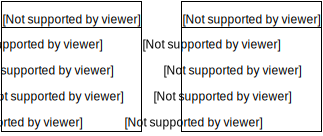
\includegraphics[scale=0.9]{img/dataTyp.pdf}
\caption{Theoretical data scheme in the metadata catalog}
\label{fig:theoDataScheme}
\end{figure}


\section{Apache Cassandra}
Apache Cassandra is a distributed database for managing large amounts of structured data 
across many commodity servers, while providing highly available service and no single point 
of failure \cite{cassandra}. Cassandra's data model is a
partitioned row store, rows are organized into tables. Each row
has an altering number of columns, which are essentially a
key-value pair, and is identified by a unique ID. Adding that Cassandra features
its own query language CQL (Cassandra Query Language) which resembles the standard SQL 
used by all relational databases, it looks like a perfect candidate for the metadata catalog.

\subsection{Developing a data model for Cassandra}

Although CQL makes it look like a relational database, the developer has to bare in mind, that
Cassandra is different. The first scheme used the altering number of columns and organized the 
data in tables, where each file or directory had its own row with metanames being the column
names and values being the column values (this model greatly resembles the theoretical data 
scheme in figure \ref{fig:theoDataScheme}) with secondary indexes over column values so that 
the query would be possible. Although the similarity with SQL would suggest otherwise, 
it turned out that this kind of indexing does not support range queries. 

After understanding more thoroughly how Cassandra works, another data model was introduced 
using most of Cassandras specific features. The key properties Cassandra guaranties are that 
rows are not divided across multiple nodes in the cluster and column keys inside the row
are sorted. Based on these two main characteristics a functioning data model was created. For  
directories row IDs are mapped on directory IDs and the model is similar to the previous one. 
Retrieving a row with given row ID is one of natively supported operations.
For files each metaname has its row, column names are meta values and column values are sets of 
file IDs of files having this metaname and value associated with them. 

\begin{table}[h]
\centering
\label{tab:fileMeta}
\begin{tabular}{|l|l|l|l|ll}
\hline
\multirow{2}{*}{Metaname A} & Value 1      & Value 2      & Value 3      & \multicolumn{1}{l|}{Value 4}      & \multicolumn{1}{l|}{Value 5}      \\ \cline{2-6}
                            & \{id,id,..\} & \{id,id,..\} & \{id,id,..\} & \multicolumn{1}{l|}{\{id,id,..\}} & \multicolumn{1}{l|}{\{id,id,..\}} \\ \hline
\multirow{2}{*}{Metaname B} & Value 1      & Value 2      & Value 3      &                                   &                                   \\ \cline{2-4}
                            & \{id,id,..\} & \{id,id,..\} & \{id,id,..\} &                                   &                                   \\ \cline{1-4}
\end{tabular}
\caption{File metadata}
\end{table}

The rows are grouped
in tables by value type, because the algorithm used to sort the
column names is unified per table. There also is an index over fileID sets, 
so that retrieving all metadata for one specific file is possible, but the scheme is 
not optimized for this operation.

\begin{listing}
\begin{minted}{sql}
CREATE TABLE file_int (
    metaname text,
    value int,
    fileid set<int>,
    PRIMARY KEY (metaname, value)
);
\end{minted}
\caption{Data structure described using CQL}
\end{listing}

In CQL this structure looks like a table with three columns and a compound primary key which
brings the main disadvantage of this approach: meta names can be queried only one at a time and
the result has to be then finalized in the DIRACs code.

\begin{listing}
\begin{minted}{sql}
SELECT fileid 
	FROM file_int 
	WHERE metaname='metaInt1' AND value>3;
\end{minted}
\caption{Example query}
\end{listing}

\section{Document databases}

Both following databases are document databases and the data scheme is fairly similar in both
of them. The metadata are stored in a JSON file with properties being meta names, indexes above
properties and key mapped to the dir or file ID.

\begin{listing}
\begin{minted}{json}
{
	'metaInt1' : 1,
	'metaStr1' : 'qwerty',
	'metaInt3' : 123
}
\end{minted}
\caption{JSON structure used in document databases}
\end{listing}

Document databases were not the first pick during developing this project, because the idea of
storing metadata in a JSON structure and then building indexes above the properties is not as
familiar as Cassandras columns, but it turned out to be even easier to use.

\subsection{MongoDB}

\subsection{Elasticsearch}

\section{Database tests}

For testing a single server was used (formerly in one of the Tier-2 computing centers, equipped
%TODO parametry storje puppet2 )
The testing data was generated trying to copy the production data structure. There is expected to
be over 10 million files with approximately different 20 meta names. %TODO odkaz na prilohu s Jirkovym mailem 
The set generated had $10 000 000 - 1$ files with $1$ to $998$ metrics associated with them 
(the generator chose a randomly $1$ to $499$ integer metrics and the same number of string ones).
The metrics names were \texttt{test[Int|Str]NNN}, where \texttt{NNN} stands for a number. The
integer values were all picked from the interval $[1;1000]$ and the string values were one of the
words from the NATO phonetic alphabet %TODO citace.
This lead to the easier composition of testing queries.

The data in form of two csv files with lines \texttt{id,metaname,value} were 63 and 59 GB big.

\subsection{Loading the big data}

Elasticsearchs python interface features a bulk load function which when fed with a generator
loads the data in chunks of 500. Unfortunately it crashes on a TimeoutException from time to 
time making the loading a rather long procedure. 

MongoDB features a command \texttt{mongoimport} which can read a file of JSON objects and load
them all. Its' pace on the test data was approximately $150-200$ entries per second. Unluckily 
the script froze from time to time so loading the whole dataset took again several days.

\chapter{NoSQL Integration into DFC}
\label{chap:NoSQL}

To prove the concept of connecting the metadata part of the DIRAC File Catalog to a NoSQL database the 
modules \texttt{fmeta} and \texttt{dmeta} that manage the the metadata in the FileCatalog service were modified.
As discussed in the previous chapter, the best available NoSQL database for this particular purpose is 
Elasticsearch. 

\section{Query Strategy}
The current query search algorithm cuts the query per element of the disjunction. With each element the Catalog
finds directories satisfying the directory part of the query, then it finds the files satisfying the file part. 
With the list of files and list of directories it filteres out the files that are not in the subtree of one of the
satisfying directories (the algorithm is described by algorithm \ref{alg:find}).

\begin{algorithm}[h]
\caption{Find files satisfying query}
\label{alg:find}
\begin{algorithmic}[1]
\Function{Find}{queryList}
	\State \textit{outFiles} = [  ]
	\ForAll{\textit{element} in \textit{queryList}}
		\State dirMeta $\leftarrow$ getDirectoryMeta(\textit{element})
		\State \textit{dirs} $\leftarrow$ findDirectories(\textit{dirMeta}) \Comment{including sub-trees}
		\State fileMeta $\leftarrow$ getFileMeta(\textit{element})
		\State \textit{files} $\leftarrow$ findFiles(\textit{fileMeta})
		\State \textit{files} $\leftarrow$ dropFilesNotInDirs(\textit{files}, \textit{dirs})
		\State \textit{outFiles}.append(\textit{files})
	\EndFor
	\State \textbf{return} removeDuplicates(outFiles)
\EndFunction
\end{algorithmic}
\end{algorithm}

The procedure is so complicated, because the metadata for directories and for files are managed by different 
modules (in the algorithm, the function \texttt{findDirectories} is in module \texttt{dmeta} and \texttt{findFiles} 
is handled by \texttt{fmeta}). This can result in unnecessary fetching of files, which are then dropped because
they happen to be located in a directory that does not satisfy the query. This is especially relevant because as
the tests done by this project suggests the query speed of Elasticsearch unlike MySQL depends mainly on the
number of hits it has to retrieve %TODO smazat tohle, pokud to bude pravda i na jednom shardu
not on the complexity of the query (see figure \ref{fig:wide}). 

The solution could be letting database engine deal 
with the complexity of the search algorithm. This would mean storing all the metadata associated with a file (its' 
own and the ones as well as the inherited from the directory structure) in the files document. This would increase
disk space (but as table \ref{tab:allDbSizes} suggests, Elasticsearch is much more space efficient when compared 
to MySQL) as well as the difficulty of metadata management. The inheritance of metadata through the directory 
structure has to be maintained when setting and unsetting them. The result would be that finding files would 
only consist of translating the metaquery from the internal representation to an Elasticsearch compatible form 
(which is now done per element in functions \texttt{findDirectories} and \texttt{findFiles}) and submitting the
query. What would be sacrificed is the fact that directory and file metadata can be handled in a completely 
different fashion.

\section{The New Implementation}

Another module was developed to create a specialized interface between the database and the metadata catalog. This 
also minimized the changes that had to be done on the current metadata managing modules (the practice where one
module manages directory metadata and another manages file metadata was left unchanged). As discussed above, the 
module stores all the metadata in one document to improve the querying speed. Setting and un-setting directory 
metadata is a rather complicate procedure, which requires fetching all the documents associated with files in
the particular sub-tree and updating them with the new metadata (respectively removing the one removed from the 
directory). 

Removing a property from a document in Elasticsearch is not one of the basically supported operations. There are 
two ways to implement it: 
\begin{enumerate}
\item Get the whole document from the database, remove the property and insert it again.
\item Submit a script that deletes the property from the document inside the database in a update-like operation.
\end{enumerate}
Because the scripting has to be enabled by the database administrator and it is not guaranteed for the DIRAC 
administrator to have administrator access to the database as well, the first approach was chose. This means that
removing a metadata from a directory that has lots of files in its sub-tree is a non-trivial operation and shall
be executed as rarely as possible. Updating and setting new metadata can be done by a simple command.

For searching the metadata managing modules from the file catalog had to be changed. The new algorithm simply 
converts the query to the correct format, submits it and reads the result.
\chapter{Users documentation}
\label{chap:user}

To start working with DIRAC 
(or the Grid in general), the user should join some 
grid Virtual Organization and obtain a Grid Certificate. 
Before a user can work with DIRAC, the user’s certificate proxy 
should be initialized and uploaded to the DIRAC ProxyManager Service \cite{DISET}.
This is done by running the command \texttt{dirac-proxy-init}. After that,
all the DIRACs' functionality is ready for use and all the actions will
be signed by the users certificate.

The primary interface to the DIRACs' file and metadata catalog
is the command line interface provided by the script
\texttt{dirac-dms-filecatalog-cli}. Commands that use the modules 
implemented by this project are \texttt{meta}, \texttt{find} 
and \texttt{dataset}.

\section{Command meta}
Command used for all the metadata manipulating operations.
The sub-commands of command meta are: \texttt{index}, \texttt{get},
\texttt{set}, \texttt{remove} and \texttt{show}.

\subsection{index}
Usage: \texttt{meta index [-d|-f|-r] <metaname> <metatype>}

Adds new metadata name to available metadata names
that the user then can assign a value to for a concrete file
or directory. The parameters \texttt{-f} and \texttt{-d} specify,
whether the new metaname will be associated with files or directories,
respectively. The \texttt{-r} parameter is used, when the user
wants to remove the metadata name. \texttt{<metatype>} can be
one of the following: int, float, string, date. User has to be
in the \texttt{dirac\_admin} group to be allowed to use this
command.

\subsection{set}
Usage: \texttt{meta set <path> <metaname> <metavalue>}

Sets a value to a metaname for a directory or file specified by
the path parameter. 

\subsection{get}

Usage: \texttt{meta get [<path>]}

Gets all user defined metadata for a directory or file specified by
the path parameter. When getting metadata for a file, it also gets
all the inherited directory metadata. When getting metadata for a
directory, the output specifies which are defined on that concrete
directory and which are inherited:
\begin{lstlisting}[language=json]
>meta get dir1
         !testDirStr : foo
          *unitFloat : 1.5
         *testDirInt : 1
\end{lstlisting}
The metadata prefixed with the \textbf{!} mark are defined on the
directory, others (prefixed with \textbf{*}) are inherited.

\subsection{remove}

Usage: \texttt{meta [remove|rm] <path> <metaname>}

Removes previously defined metaname for a directory or file
specified by the path parameter.

\subsection{show}

Usage: \texttt{meta show}

Shows all the available metadata names, divides them between the
file and directory metadata and supplies the type.

\section{Command find}

Usage: \texttt{find [-q] [-D] <path> <metaQuery>}

Finds all files satisfying the given metadata query. When the
command is invoked it parses the query and, unless the \texttt{-q}
parameter prints is used, prints it out in its internal
representation. After the query results return, the list of all
the files satisfying it is printed out. When the \texttt{-D}
parameter is used, the command prints only the directories
that contain the files that satisfy the metaquery.

\section{Command dataset}
Command used for all the operations involving the dataset
functionality. Sub-commands are \texttt{add, annotate, check,
download, files, freeze, locate, overlap, release, replicate, rm,
show, status} and \texttt{update}.

\subsection{add}

Usage: \texttt{dataset add [-f] <dataset\_name> <meta\_query>}

Adds a new dataset containing all files satisfying the query
supplied by the \texttt{<meta\_query>} parameter. In the
\texttt{<dataset\_name>} the user specifies the path to where the
dataset should be located. When the \texttt{-f} in used, the
dataset is immediately frozen.

\subsection{annotate}

Usage: \texttt{dataset annotate [-r] <dataset\_name> <annotation>}

Adds annotation to a dataset. There is no indexing involving
annotations, they are just for the user. The annotation is a string
up to 512 characters long. When the \texttt{-r} parameters is used,
the annotation is removed from specified dataset. A dataset can
have only one annotation.

\subsection{check}

Usage: \texttt{dataset check <dataset\_name> [<dataset\_name>]*}

Checks the correctness of the cached information about the dataset.
It can be supplied with one dataset, or a list of dataset names
separated with spaces. The information can be outdated by recent
file addition or removal in the file catalog and can be updated
using the sub-command \texttt{update}.

\subsection{download}

Usage: \texttt{dataset download <dataset\_name>  [-d <target\_dir>]
[<percentage>]}

Invokes download of the dataset files. If the \texttt{percentage}
parameter is used, a subset of the datasets files are downloaded
that its whole size is approximately the percentage of the size
of the whole dataset. Unless the \texttt{-d} parameter supplies the
target directory, the current working directory is used. The
command creates a directory with the same name as the dataset and
all the files are saved there.

\subsection{files}

Usage: \texttt{dataset files <dataset\_name>}

Lists out all the files that the specified dataset groups. In case
of a frozen dataset, the files saved in the database associated
to the dataset are listed. When the dataset is dynamic, the command
returns the same result, as using the \texttt{find} command with
the datasets metaquery.

\subsection{freeze}

Usage: \texttt{dataset freeze <dataset\_name>}

Changes the status of a dataset to frozen. All the files that
satisfy the datasets metaquery at the moment of the command
invocation are associated with the dataset. For releasing the
dataset, the sub-command \texttt{release} is used.

\subsection{locate}

Usage: \texttt{dataset locate <dataset\_name>}

Shows the distribution of the dataset files over the storage
elements providing the absolute size and percentage of the dataset
size used per storage element.

\subsection{overlap}

Usage: \texttt{dataset overlap <dataset\_name1> <dataset\_name2> }

Checks if the two datasets have the same files. The metaqueries are
checked first so that when there cannot be files satisfying both,
the check does not compare lists of files.

\pagebreak

\subsection{release}

Usage: \texttt{dataset release <dataset\_name>}

Changes the status of a dataset to dynamic. All the records
associating concrete files to the dataset are deleted from the
database. For freezing the dataset, the sub-command \texttt{freeze}
is used, however if there were files added to the file catalog that
satisfy the datasets metaquery after the dataset was frozen, the
subset of files satisfying the metaquery not including those files
cannot be recreated after releasing the dataset.

\subsection{replicate}

Usage: \texttt{dataset replicate <dataset\_name> <SE>}

Initiates a bulk replication of the datasets files to a storage
element specified by the parameter \texttt{SE}. The replication
is handled by the Request Management System.

\subsection{rm}

Usage: \texttt{dataset rm <dataset\_name>}

Deletes the dataset from the file catalog. If the dataset is
frozen, its files are cross-checked with all other frozen datasets
and if there are some files that are grouped by the deleted dataset
only, the user is offered the option to delete those files from the
file catalog. The deletion is handled by the Request Management
System.

\subsection{show}

Usage: \texttt{dataset show [-l] [<dataset\_name>]}

Lists the names of all the existing datasets. When the \texttt{-l}
option is used, other data about the datasets are printed as well.
When a \texttt{<dataset\_name>} is provided, the command restricts
itself to this dataset.

\subsection{update}

Usage: \texttt{dataset update <dataset\_name> [<dataset\_name>]*}

Updates the cached parameters for a dataset or for a space
separated list of datasets.

\pagebreak

\subsection{status}

Usage: \texttt{dataset status <dataset\_name> [<dataset\_name>]*}

Prints details about a specified dataset or space separated list of
datasets.

\begin{lstlisting}[language=json]
> dataset status testDataset
testDataset:
========
    Key              Value
======================================================
  1 NumberOfFiles    13
  2 MetaQuery        testDirInt = 1
  3 Status           Dynamic
  4 DatasetHash      A89F08D23140960BDC5021532EF8CC0A
  5 TotalSize        61562
  6 UID              2
  7 DirID            5
  8 OwnerGroup       dirac_admin
  9 Owner            madam
 10 GID              1
 11 Mode             509
 12 ModificationDate 2015-09-24 11:50:28
 13 CreationDate     2015-09-24 11:50:28
 14 DatasetID        71
\end{lstlisting}


\chapter*{Conclusion}
\addcontentsline{toc}{chapter}{Conclusion}

This project successfully added dataset support to the DIRAC File Catalog making DIRAC even more 
versatile. Closely coupled with the dataset functionality went the development of the new MetaQuery
class that extended the metaquery language by adding more logical operators. The new MetaQuery also
supports normalization and optimization of the query input opening new possibilities for future usage
in the DIRAC Data Management system as well as the Workflow Management system. 

This project also tackled the problem of storing metadata. To solve it a couple of NoSQL databases were tested
on sample data similar to what DIRAC production metadata. The tests proved that connecting the 
metadata part of DFC to a NoSQL database could improve query performance, especially on more complex
queries. 

To prove the concept of connecting a NoSQL database to DIRAC a new module was developed to provide 
a interface between DFC and the database. As the back-end database Elasticsearch, the database performing 
best in the conducted tests was used. This conveniently moved the complexity from query execution to the database 
and matadata management.

%%% Seznam použité literatury
%%% Seznam použité literatury je zpracován podle platných standardů. Povinnou citační
%%% normou pro bakalářskou práci je ISO 690. Jména časopisů lze uvádět zkráceně, ale jen
%%% v kodifikované podobě. Všechny použité zdroje a prameny musí být řádně citovány.

\def\bibname{Bibliography}
\begin{thebibliography}{99}
\addcontentsline{toc}{chapter}{\bibname}

%\bibitem{lamport94}
%  {\sc Lamport,} Leslie.
%  \emph{\LaTeX: A Document Preparation System}.
%  2. vydání.
%  Massachusetts: Addison Wesley, 1994.
%  ISBN 0-201-52983-1.

\bibitem{happyBday}
	Hayes, Jacqui: 
	\emph{Happy 10th Birthday, WLCG!} [online]
	International Science Grid This Week [cit. 2014-09-18]
	\texttt{www.isgtw.org/feature/happy-10th-birthday-wlcg}

\bibitem{TGrid}
	\emph{The Grid: A system of tiers} [online] 
	CERN [cit. 2014-09-18]
	\texttt{home.web.cern.ch/about/computing/grid-system-tiers}

\bibitem{GriCom}
	\emph{Grid Computing - Technology and Applications, Widespread Coverage and New Horizons.} 
	edited by Maad, Soha; InTech, 2012.
	ISBN 978-953-51-0604-3

\bibitem{UI}
	\emph{User Interfaces} [online] 
	EGIWiki [cit. 2014-09-29]
	\texttt{wiki.egi.eu/wiki/User\_Interfaces}
	
\bibitem{ATLASDDM1}
	GARONNE, Vincent, Graeme A STEWART, Mario LASSNIG, Angelos MOLFETAS, Martin BARISITS, Thomas BEERMANN, 
	Armin NAIRZ, Luc GOOSSENS, Fernando BARREIRO MEGINO, Cedric SERFON, Danila OLEYNIK a Artem PETROSYAN. 
	The ATLAS Distributed Data Management project: Past and Future. 
	\textit{Journal of Physics: Conference Series}. 2012-12-13, vol.~396, issue 3, s.~032045-. 
	DOI: 10.1088/1742-6596/396/3/032045. 
	
\bibitem{ATLAS-Rucio}
	GARONNE, V, R VIGNE, G STEWART, M BARISITS, T B EERMANN, M LASSNIG, C SERFON, L GOOSSENS a A NAIRZ. 
	Rucio – The next generation of large scale distributed system for ATLAS Data Management. 
	\textit{Journal of Physics: Conference Series}. 2014-06-11, vol.~513, issue 4, s.~042021-. 
	DOI: 10.1088/1742-6596/513/4/042021.

\bibitem{Dir1}
	\emph{DIRAC overview} [online] 
	DIRAC documentation [cit. 2014-09-18]
	\texttt{diracgrid.org/files/docs/Overview/index.html}
	
\bibitem{Dir2}
	\emph{DIRAC} [online] 
	The Interware [cit. 2015-05-06]
	\texttt{diracgrid.org}
		

\end{thebibliography}


%%% Tabulky v bakalářské práci, existují-li.
\chapwithtoc{List of Tables}



%%% Použité zkratky v bakalářské práci, existují-li, včetně jejich vysvětlení.
\chapwithtoc{List of Abbreviations}
\begin{description}
	\item[CERN] European Organization for Nuclear Research (name derived from Conseil Européen pour la Recherche 
	Nucléaire) -- European research organization that operates the largest particle physics laboratory in the 	
	world.
	\item[LHC] Large Hadron Collider -- the world's largest and most powerful particle collider built by CERN
	\item[WLCG] The Worldwide LHC Computing Grid -- global collaboration of more than 170 computing 
	centres in 42 countries, linking up national and international grid infrastructures
	
	\item[CLI] Command Line Interface -- means of interacting with a computer program
	
	\item[DNF] Disjunctive Normal Form -- standard form of a logical formula, which is a disjunction of 
	conjunctive clauses

	\item[DIRAC] The Distributed Infrastructure with Remote Agent Control -- middleware developed by one of the 
	CERNs' collaborations
	\item[DFC] DIRAC File Catalog -- file catalog service in the DIRAC middleware 
	\item[LFC] LCG File Catalog -- file catalog provided by CERN IT department 
	
	\item[LFN] Logical File Name -- name of the file displayed to a file catalog user 
	\item[PFN] Physical File Name -- complete file URL 
	
	\item[CQL] Cassandra Query Language -- the primary language for communicating with the Cassandra database
	
	\item[WT] WiredTiger -- MongoDB storage engine, newly available in version 3.0
	
	\item[SRM] Storage Resource Managers -- middleware software modules managing available storage resource 
\end{description}

%%% Přílohy k bakalářské práci, existují-li (různé dodatky jako výpisy programů,
%%% diagramy apod.). Každá příloha musí být alespoň jednou odkazována z vlastního
%%% textu práce. Přílohy se číslují.
%\chapwithtoc{Attachments}

\begin{appendix}
\renewcommand{\chaptermark}[1]{\markboth{Appendix \thechapter \hspace{0.1mm}\ #1}{}}
\addappheadtotoc
\chapter{Queries} \label{app:queries}

This attachment lists the set of queries, which was used to get a basic benchmark of the databases performance.
The queries are written in JSON form for convinience: a one level JSON is essentially a serialized form of the 
python dictionary data structure. When creating a meaningful query from the JSON the following algorithm is used:

\begin{itemize}
	\item if the current key contains the substring \texttt{Int}, then according to the projects' 
		conventions the field represents an integer typed metafield. The query condition in this case is 
		\texttt{[key] > [value]},
	\item otherwise (key contains substring \texttt{Str}) the field represents a string metafield adn the condition
		is \texttt{[key] = [value]}.
\end{itemize}


\begin{lstlisting}

{'testInt2': 844, 'testInt8': 406}

{'testInt2': 125, 'testInt7': 101}

{'testInt5': 270, 'testInt6': 267}

{'testInt1': 154, 'testInt2': 69, 'testInt7': 305}

{'testInt2': 260, 'testInt4': 731, 'testInt5': 873}

{'testInt1': 185, 'testInt5': 389, 'testInt7': 561}

{'testInt2': 19,
 'testInt3': 745,
 'testInt5': 600,
 'testInt7': 321}

{'testInt1': 330,
 'testInt2': 168,
 'testInt3': 477,
 'testInt7': 515}

{'testInt2': 809,
 'testInt4': 339,
 'testInt7': 848,
 'testInt8': 562}

{'testInt5': 593, 'testStr1': 'foxtrot'}

{'testInt2': 258, 'testStr2': 'yankee'}

{'testInt6': 805, 'testStr3': 'tango'}

{'testInt4': 467, 'testInt5': 364, 'testStr2': 'juliet'}

{'testInt5': 85, 'testInt8': 385, 'testStr1': 'juliet'}

{'testInt3': 506, 'testInt5': 840, 'testStr2': 'victor'}

{'testInt2': 645,
 'testInt4': 57,
 'testInt5': 309,
 'testStr2': 'kilo'}

{'testInt1': 794,
 'testInt4': 190,
 'testInt8': 663,
 'testStr3': 'juliet'}

{'testInt2': 621,
 'testInt4': 495,
 'testInt8': 558,
 'testStr3': 'whiskey'}

{'testInt1': 833,
 'testInt6': 807,
 'testInt7': 336,
 'testInt8': 58,
 'testStr3': 'sierra'}

{'testInt3': 943,
 'testInt5': 292,
 'testInt6': 762,
 'testInt7': 160,
 'testStr1': 'charlie'}

{'testInt5': 339,
 'testInt6': 918,
 'testInt7': 752,
 'testInt8': 789,
 'testStr3': 'mike'}

{'testInt8': 157, 'testStr1': 'kilo', 'testStr2': 'hotel'}

{'testInt6': 347, 'testStr1': 'papa', 'testStr2': 'india'}

{'testInt3': 109, 'testStr1': 'victor', 'testStr3': 'juliet'}

{'testInt5': 240,
 'testInt6': 578,
 'testStr1': 'delta',
 'testStr3': 'golf'}

{'testInt3': 131,
 'testInt4': 160,
 'testStr1': 'kilo',
 'testStr2': 'tango'}

{'testInt3': 487,
 'testInt8': 856,
 'testStr1': 'charlie',
 'testStr3': 'whiskey'}

{'testInt4': 443,
 'testInt5': 103,
 'testInt7': 540,
 'testStr2': 'india',
 'testStr3': 'golf'}

{'testInt3': 303,
 'testInt7': 200,
 'testInt8': 866,
 'testStr1': 'foxtrot',
 'testStr3': 'golf'}

{'testInt1': 532,
 'testInt4': 371,
 'testInt6': 155,
 'testStr2': 'india',
 'testStr3': 'yankee'}

{'testInt1': 479,
 'testInt2': 432,
 'testInt3': 915,
 'testInt8': 33,
 'testStr1': 'quebec',
 'testStr2': 'alpha'}

{'testInt1': 826,
 'testInt4': 802,
 'testInt5': 824,
 'testInt8': 874,
 'testStr1': 'juliet',
 'testStr2': 'golf'}

{'testInt2': 604,
 'testInt4': 791,
 'testInt5': 354,
 'testInt6': 668,
 'testStr1': 'juliet',
 'testStr2': 'xray'}

\end{lstlisting}


\chapter{MongoDB explain index} \label{app:MDB}

This appendix lists output of the \texttt{db.collection.explain.find()} command applied to 
one of the queries from the testing set. The rewriting of that query can be seen in the first listing, the output
in the second one. 

\begin{minted}{sql}
SELECT FileID FROM Metas 
	WHERE testInt5.Value > 364 
	AND testStr2.Value='juliet' 
	AND testInt4.Value > 467;
\end{minted}

In the beginning the query planner writes some basic information about the search (the names \texttt{namespace},
\texttt{parsedQuery}, etc.). Then the details of the query plan selected by the optimizer are listed in name
\texttt{winningPlan}. The stage \texttt{FETCH} describes retrieving documents, in this particular case the documents
are filtered so that the constraints that are minor according to the query planer are fulfilled. Then in the next
stage \texttt{IXSCAN} the index is scanned. In this case the index over the property \texttt{testStr2} was chosen.
After the winning plan, two more rejected plans are described. These plans differ from the winning one by using a 
different index. In the end some information about the current server was printed by the command, but was not
included here because it has no relevance for this problem.

\begin{minted}{json}
{
  "queryPlanner": {
    "plannerVersion": 1,
    "namespace": "fcall.files",
    "indexFilterSet": false,
    "parsedQuery": {
      "$and": [
        {
          "testStr2": {
            "$eq": "juliet"
          }
        },
        {
          "testInt4": {
            "$gt": 467
          }
        },
        {
          "testInt5": {
            "$gt": 364
          }
        }
      ]
    },
    "winningPlan": {
      "stage": "FETCH",
      "filter": {
        "$and": [
          {
            "testInt4": {
              "$gt": 467
            }
          },
          {
            "testInt5": {
              "$gt": 364
            }
          }
        ]
      },
      "inputStage": {
        "stage": "IXSCAN",
        "keyPattern": {
          "testStr2": 1
        },
        "indexName": "testStr2_1",
        "isMultiKey": false,
        "direction": "forward",
        "indexBounds": {
          "testStr2": [
            "[\"juliet\", \"juliet\"]"
          ]
        }
      }
    },
    "rejectedPlans": [
      {
        "stage": "FETCH",
        "filter": {
          "$and": [
            {
              "testStr2": {
                "$eq": "juliet"
              }
            },
            {
              "testInt4": {
                "$gt": 467
              }
            }
          ]
        },
        "inputStage": {
          "stage": "IXSCAN",
          "keyPattern": {
            "testInt5": 1
          },
          "indexName": "testInt5_1",
          "isMultiKey": false,
          "direction": "forward",
          "indexBounds": {
            "testInt5": [
              "(364.0, inf.0]"
            ]
          }
        }
      },
      {
        "stage": "FETCH",
        "filter": {
          "$and": [
            {
              "testStr2": {
                "$eq": "juliet"
              }
            },
            {
              "testInt5": {
                "$gt": 364
              }
            }
          ]
        },
        "inputStage": {
          "stage": "IXSCAN",
          "keyPattern": {
            "testInt4": 1
          },
          "indexName": "testInt4_1",
          "isMultiKey": false,
          "direction": "forward",
          "indexBounds": {
            "testInt4": [
              "(467.0, inf.0]"
            ]
          }
        }
      }
    ]
  },
  "ok": 1
}
\end{minted}
\end{appendix}

\openright
\end{document}
